\chapter{Supplementary Materials}
\section{The brain and its main structures}
\begin{itemize}
 \item \textit{basal ganglia}: collection of structures located deep within the brain that are involved in the control of movement, particularly in the initiation and suppression of movements.
 \item the \textit{striatum}: involved in the control of movement, it sends output to the motor cortex. 
 \item  \textit{brainstem} composed of the midbrain, pons and medulla, it connects the brain to the spinal cord
 the \item the \textit{locus coeruleus} (inside the pons, involved in the regulation of attention and arousal. It releases the neurotransmitter norepinephrine, which can modulate the activity of other brain regions).
 \item the \textit{basal forebrain} (involved in the regulation of attention, learning, and memory. It contains several different nuclei that release the neurotransmitter acetylcholine)
 \item the \textit{nucleus basalis of Meyner} (The nucleus basalis of Meynert is a group of neurons located in the basal forebrain that release acetylcholine and play an important role in attention and memory)
 \item the \textit{amygdala} (in the temporal lobe, involved in the processing of emotions, particularly fear and anxiety)
 \item the \textit{raphe nuclei} (collection of nuclei located in the brainstem that release the neurotransmitter serotonin. They are involved in the regulation of mood, sleep, and appetite)
 \item the \textit{substantia niagra} (structure located in the midbrain that is involved in the control of movement. It releases the neurotransmitter dopamine, which is important for the initiation and control of voluntary movements.)
 \item the \textit{ventral tegmental area} (The ventral tegmental area is a group of neurons located in the midbrain that release dopamine and play an important role in reward processing and motivation.)
 \item the \textit{hypothalamus} (small structure located near the base of the brain that plays a crucial role in regulating many physiological processes, such as hunger, thirst,).
\end{itemize}


\newpage
% ----------------------------------------------
% ----------------------------------------------
%
%
%               PHASE PLANE ANALYSIS
%
%
% ----------------------------------------------
% ----------------------------------------------

\section{Phase plane analysis: a powerful tool}
\subsubsection{Mathematical reminders}
This section is a general toolbox to understand non-linear systems analysis, based on the manuscript I wrote for the lecture 'Introduction to signals and systems' (fr: introduction aux signaux et systèmes, a lecture taught in second year of Bachelor at the Faculty of Applied Sciences at the University of Liège) \textcolor{red}{REF}. 

We start with a non-linear system of two variables $x_1$ and $x_2$ such as : 
\begin{equation*}
\left\{
    \begin{array}{lllllll}
        \dot{x}_1 &=& f_1(x_1,x_2)\\
        \dot{x}_2 &=& f_2(x_1,x_2) 
    \end{array}
\right.
\end{equation*}
\textbf{Graphical analysis in the phase plane}\\
Without solving complicated math, the phase plane allows to understand globally the dynamics of the systems. The phase portrait is a 2D plane and the horizontal axis is associated with the $x_1$ and the vertical axis is $x_2$.

We define the \textit{nullclines} which are defined as the locus of points where one of the derivative is null:
\begin{equation*}
\left\{
    \begin{array}{lllllll}
        x_1\mbox{-nullcline}: \dot{x}_1 =0 \rightarrow f_1(x_1,x_2) = 0  \\
        x_2\mbox{-nullcline}: \dot{x}_2 =0 \rightarrow f_2(x_1,x_2) = 0 \\
    \end{array}
\right.
\end{equation*}
The intersections between the two nullclines where $\dot{x}_1=0$ and $\dot{x}_2=0$ simultaneously defines the \textit{fixed points}: $(x_1^*,x_2^*)$. 

At each point on the plane, we can compute
\begin{equation*}
\left\{
    \begin{array}{lllllll}
        \dot{x}_1^* &=& f_1(x_1^*,x_2^*)\\
        \dot{x}_2^* &=& f_2(x_1^*,x_2^*) 
    \end{array}
\right.
\end{equation*}
where $\dot{x}_1^*$ gives the horizontal velocity and  $\dot{x}_2^*$ gives the vertical velocity. The resulting vector is the velocity at the given point in the plane. We can draw these vectors for plenty of points in the plane which brings out the \textit{vector field}. By analogy, we imagine a piece of wood on a water, the vector field simply provides the direction of the current, the fixed points are locations where the piece of wood remains fixed. 

To determine the stability of the fixed points, we watch the direction of the fields. When all the lines converge towards this point, it is a \textit{stable} fixed point. By contrast, if all the line diverge, it is a \textit{unstable} fixed point. We can also differenciate if the lines rotates towards the fixed points; it defines a stable spirale while if its direclty converges towards the point it is stable node. A similar reasoning permits to observe unstable spirale or unstable node. We can also define limit case such as center where the vector field is never converging and diverging from the node and saddle node where the vector field is attracted in one direction and repulse in the other direction. 

As you can see, this analysis provides a good way to study non linear system without solving all the differential equations and without doing any computations. \\
~\\
\textbf{Analytical analysis in the phase plane}\\
We can also determine the stability of the phase plane via analytic computations. We introduce the Jacobian matrix: 
\begin{align*}
    A &=  \begin{pmatrix}  \dfrac{\partial f_1}{\partial x_1} & \dfrac{\partial f_1}{\partial x_2} \\  \dfrac{\partial f_2}{\partial x_1} & \dfrac{\partial f_2}{\partial x_2}  \end{pmatrix}
\end{align*}

Then the eigenvalues of the Jacobian evaluated at the fixed points give the nature and stability of the fixed points. Here we consider a 2D system, the stability can be determined based on the determinant and the trace of the jacobian following Figure \ref{fig:strogatz}.

\begin{figure}[h!]
    \centering
    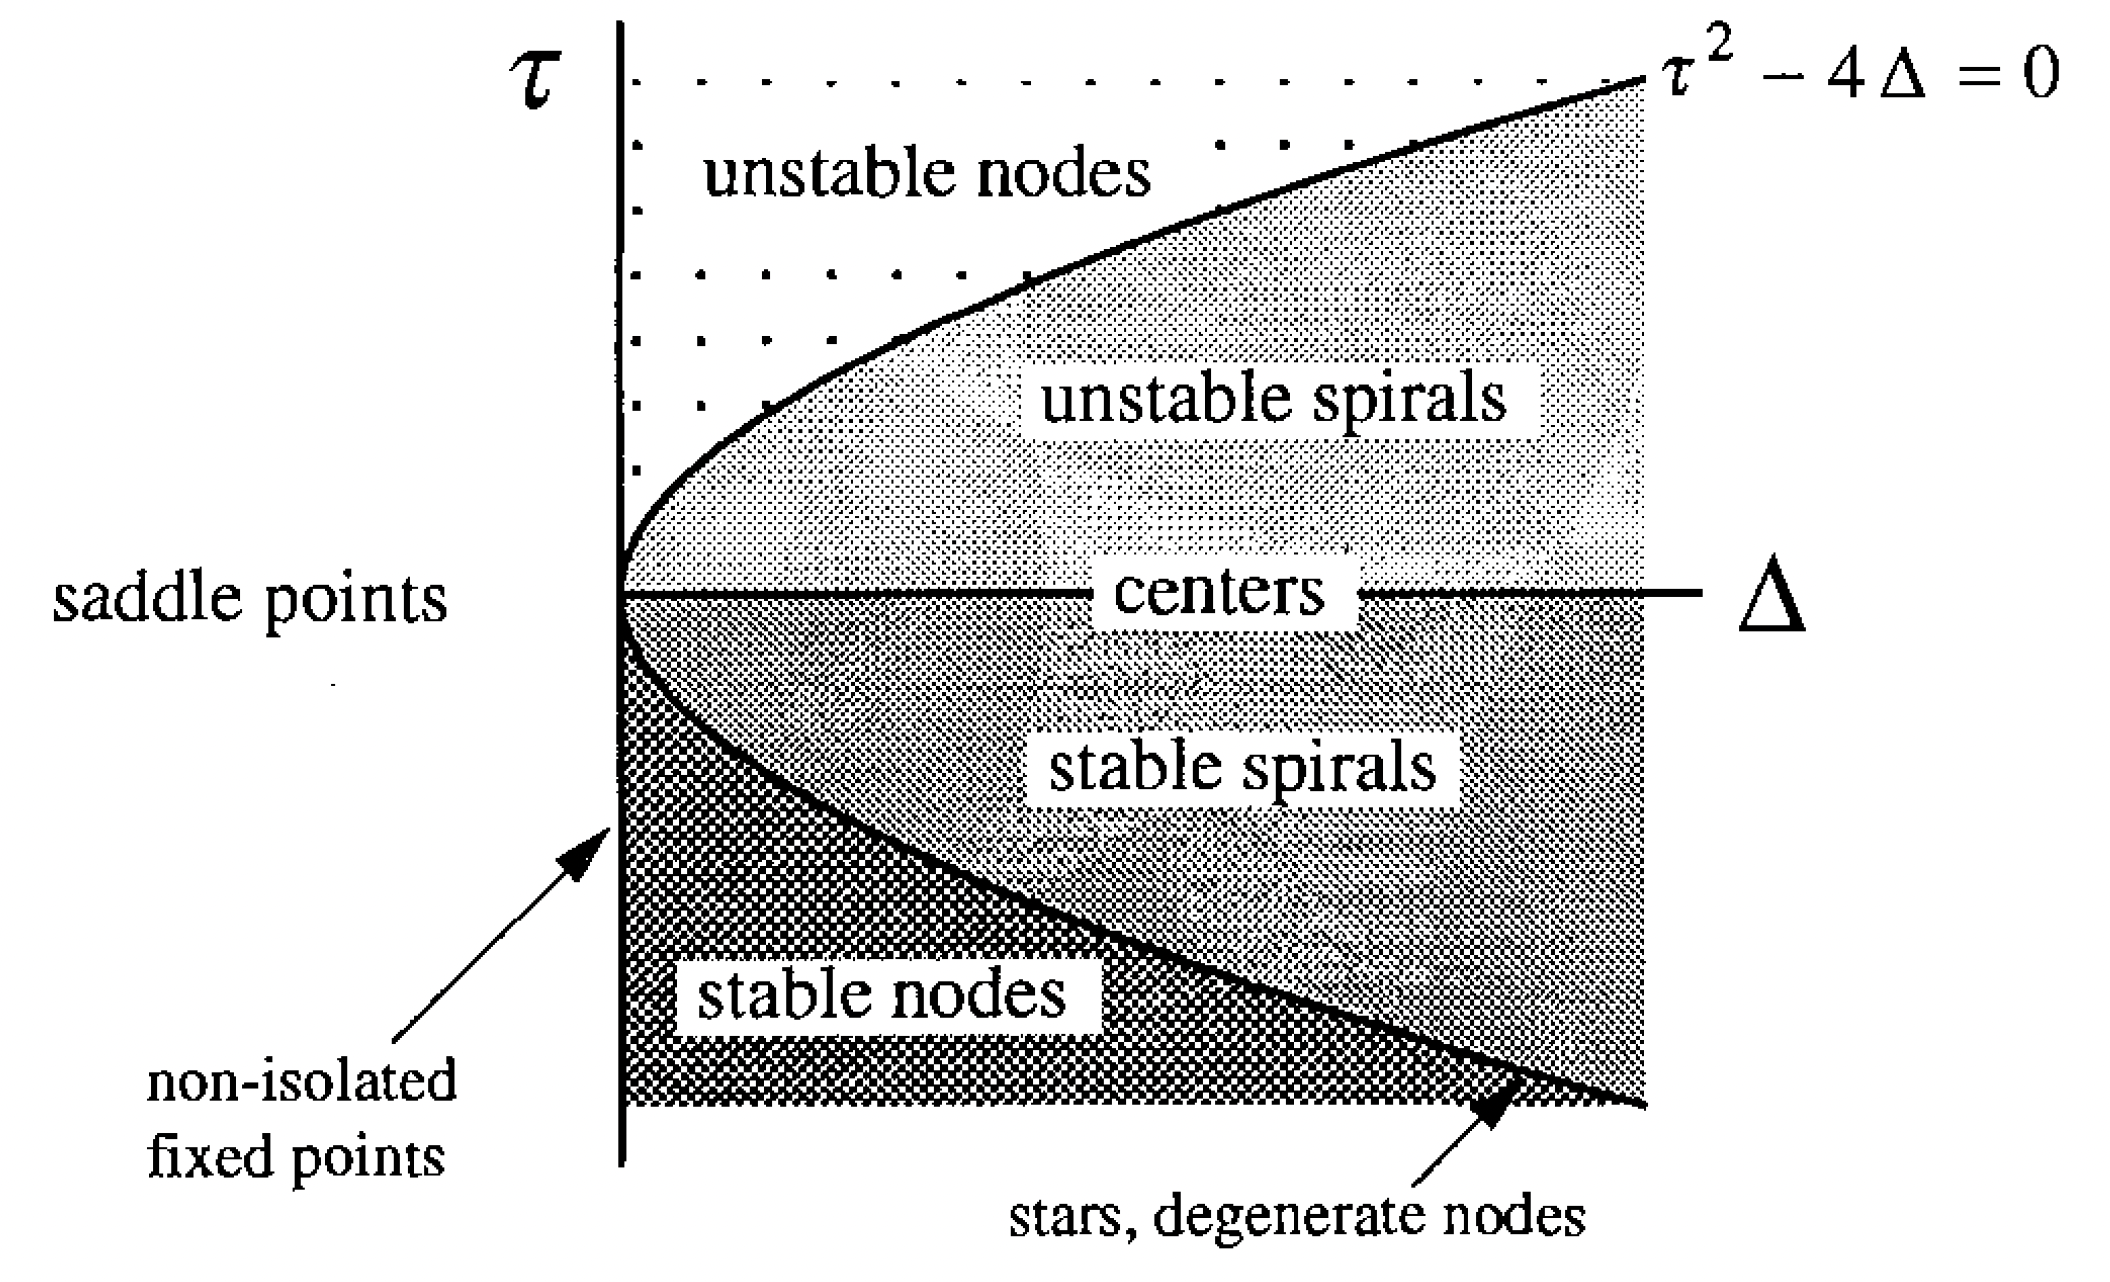
\includegraphics[scale=0.3]{latex/fig/Methods/Strogatz.png}
    \caption{The stability of the fixed points in a 2D system is defined by the values of the trace ($\tau$) and the determinant ($\Delta$) of the jacobian evaluated at the fixed points \citep{strogatz_nonlinear_2015}}
    \label{fig:strogatz}
\end{figure}


\begin{pinkshaded}
\begin{center}
\textbf{Notions clés}\\
\end{center}
~\\
\begin{tabular}{l| l l}
    Approche &\textbf{Globale | Graphique}  & \textbf{Locale | Mathématique} \\
     &tracer $\dot{x} = f(x)$ & équation $\dot{x} = f(x)$ \\
    Points fixes & intersection avec l'axe x & résoudre équation:$f(x)=0 \rightarrow x^*=...$\\
    Stabilité & tracer le champ de vecteur & étudier le signe de la dérivée première \\
    & $\dot{x}>0: \rightarrow$& (i) calcul $f'(x)$\\
    & $\dot{x}<0: \leftarrow$& (ii) remplacer $x$ par $x*$: $f'(x^*)$\\
    \textit{stable} &     $\rightarrow \bullet \leftarrow$ &  $f'(x^*)<0$ (pente négative)\\
    \textit{instable}&    $\leftarrow \circ \rightarrow$ &  $f'(x^*)>0$ (pente positive)\\
\end{tabular}
\end{pinkshaded}



% -------------------------
%
%
%       SI Article PLOS
%
%-------------------------

\begin{comment}
\chapter{Supplementary Materials}

\section{Plos Article}
\section*{Supporting information}

% Include only the SI item label in the paragraph heading. Use the \nameref{label} command to cite SI items in the text.

\paragraph{S1}
\label{S1_Video}
{\bf Video. Membrane voltage evolution during a hyperpolarized-induced bursting (top) and its associated phase portrait considering a \textit{fast} activation of T-type calcium channel (bottom).} V-(resp. V-s) nullcline is skteched in blue (resp. green).  The trajectory is marked by round circles. The simulation is shown for the reduced model 1 (Video associated to Fig~\ref{fig:6} (left)).

\paragraph{S2}
\label{S2_Video}
{\bf Video. Membrane voltage evolution during a hyperpolarized-induced bursting (top) and its associated phase portrait for a \textit{slow} activation of T-type calcium channel (bottom).} V-(resp. V-s) nullcline is skteched in blue (resp. green).  The trajectory is marked by round circles. The simulation is shown for the reduced model 1 (Video associated to Fig~\ref{fig:6} (center)).

\paragraph*{S3}
\label{S3_Video}
{\bf Video. Membrane voltage evolution during a hyperpolarized-induced bursting (top) and its associated phase portrait for a \textit{ultraslow} activation of T-type calcium channel (bottom).} V-(resp. V-s) nullcline is skteched in blue (resp. green).  The trajectory is marked by round circles. The simulation is shown for the reduced model 1 (Video associated to Fig~\ref{fig:6} (right)).

\paragraph{S4}
\label{S4_Video}
{\bf Video. Phase portrait evolution as a function of the T-type calcium channel activation kinetics } V-(resp. V-s) nullcline is skteched in blue (resp. green). The multiplicative factor of the T-type calcium channel activation time constant is indicated by $\eta$.  Apparition of the lower branch in the V-nullcline when the activation decelerates. Then, the lower branch disappears into a hourglass shape. Results shown for the reduced model 1. Similar phase portraits evolution of the reduced models 2, 5' and 6' are available on \url{http://www.montefiore.ulg.ac.be/~guilldrion/Files/Jacquerie2021_codes.zip} (in the folder "video").

\paragraph*{S5}
\label{S5_Video}
{\bf Video. Membrane voltage evolution during a hyperpolarized-induced bursting (top) and its associated phase portrait at the nominal value of the membrane capacitance (bottom).} V-(resp. V-s) nullcline is skteched in blue (resp. green).  The trajectory is marked by round circles (Video associated to Fig~\ref{fig:7}A (left)).

\paragraph*{S6}
\label{S6_Video}
{\bf Video. Membrane voltage evolution during a hyperpolarized-induced bursting (top) and its associated phase portrait when the membrane capacitance is scaled by 1/3 (bottom).} V-(resp. V-s) nullcline is skteched in blue (resp. green).  The trajectory is marked by round circles (Video associated to Fig~\ref{fig:7}A (right)).

\paragraph*{S7}
\label{S7_Video}
{\bf Video. Membrane voltage evolution during a hyperpolarized-induced bursting (top) and its associated phase portrait at the nominal value of the membrane capacitance (bottom).} V-(resp. V-s) nullcline is skteched in blue (resp. green).  The trajectory is marked by round circles (Video associated to Fig~\ref{fig:7}B (left)).

\paragraph*{S8}
\label{S8_Video}
{\bf Video. Membrane voltage evolution during a hyperpolarized-induced bursting (top) and its associated phase portrait when the membrane capacitance is scaled by 1/3 (bottom).} V-(resp. V-s) nullcline is skteched in blue (resp. green).  The trajectory is marked by round circles (Video associated to Fig~\ref{fig:7}B (right)).




\paragraph*{S1}
\label{S1_Supplementary_Material}
{\bf Supplementary Material.} \textbf{A:} Quantification of the firing pattern properties. \textbf{B:}  Simulation of the reduced models not exhibited in the Results.  \textbf{C:} Model description and their parameter values.  \textbf{D:} 
Ionic channel description: steady-state functions and time constants of the gating variables.  \textbf{E:} Description of reduced models and their parameter values. 
\end{comment}